% Verification wrapper only; the delivered transcription is a fragment.
\documentclass[11pt]{article}
\usepackage[T1]{fontenc}
\usepackage[utf8]{inputenc}
\usepackage{amsmath,amssymb,tikz-cd,xcolor}
\usepackage[paperwidth=32cm,paperheight=42cm,margin=1.5cm]{geometry}
\setlength{\parindent}{0pt}
\setlength{\parskip}{5pt}
\newcommand{\cotefile}[1]{}
\newcommand{\scanpage}[1]{\clearpage\section*{Scan #1}}
\newcommand{\mspage}[1]{\textbf{#1}\par}
\newcommand{\deleted}[1]{{\color{gray}#1}}
\newcommand{\inserted}[1]{{\color{blue}#1}}
\newcommand{\margin}[1]{\par{\color{teal}#1}\par}
\newcommand{\uline}[1]{#1}
\newcommand{\uuline}[1]{#1}
\newcommand{\diagram}[1]{\par\noindent#1\par}
\renewcommand{\figure}[1]{\par\noindent#1\par}
\def\firstchoice#1|#2\stopchoice{#1}
\newcommand{\unsure}[1]{\firstchoice#1|\stopchoice}
\newcommand{\illegible}[1]{[unreadable #1 word(s)]}
\begin{document}
\cotefile{68}
\scanpage{33}
% archive foliation: 32
\[
\left\{\begin{aligned}
G\cap(C\setminus C_0)&=\unsure{G^\times|G^*}\\
P\cap(C\setminus C_0)&=\unsure{P^*|P^\times}\\
C\setminus(G\cup P)&=N
\end{aligned}\right.
\qquad\text{(positions nulles, i.e. gagnantes pour aucun des deux joueurs)}
\]
Une position $x$ sera encore dite \uline{gagnante} (resp. \uline{perdante}) si $x\in G$ (resp. $x\in P$) --- cette terminologie coïncide avec la précédente si $x\notin C_0$. On aura, posant
\[
\deleted{\unsure{G(j)=\{x\in}}
\]
\[
\hat C(j)=\{x\in C\mid\unsure{\hat\alpha}(x)=j\}
\]
(de sorte que $C$ \unsure{apparait|apparaît} comme réunion disjointe des deux ens. $\hat C(j)$, $j\in J$),
\[
\left\{\begin{aligned}
G(j)\cap\hat C(j)&=\deleted{\unsure{\hat\alpha}}\ \hat C(j)\cap G\\
G(j)\cap\hat C(\bar j)&=\hat C(\bar j)\cap P
\end{aligned}\right.
\]
donc \inserted{les} $G(j)$ $(j\in J)$ se \unsure{reconstituent} à partir de $\unsure{\hat\alpha}$ et des ensembles $G,P$.

On aura, pour $x\in C\setminus C_0$
\[
\begin{aligned}
x\in G&\Longleftrightarrow\exists y\in R(x)\ \inserted{\text{tel que}}\ y\in P
&&\text{i.e. }R(x)\cap P\ne\varnothing\\
x\in P&\Longleftrightarrow\forall y\in R(x),\ \text{on a }y\in G
&&\text{i.e. }R(x)\unsure{\in|\subset}G
\end{aligned}
\]
i.e.
\[
\begin{aligned}
G\cap(C\setminus C_0)\deleted{\unsure{G}}&=\{x\in C\setminus C_0\mid R(x)\cap P\ne\varnothing\}\\
P\cap(C\setminus C_0)&=\{x\in C\setminus C_0\mid R(x)\subset G\}
\end{aligned}
\]

\scanpage{34}
% archive foliation: 33
\uline{Proposition} \unsure{Soit} $(C,R,J,\hat\alpha,G_0:J\longrightarrow\unsure{\mathcal P|P}(C_0))$ un jeu de position à deux joueurs jouant alternativement, $G\subset C$ et $P\subset C$, l'ens des positions gagnantes resp. perdantes. Soient $\widetilde G,\widetilde P$ deux parties de $C$ ayant les propriétés suivantes
\[
\begin{aligned}
1)\quad&\forall x\in\widetilde G,\quad\exists y\in R(x)\quad\text{tel que }y\in\widetilde P\\
2)\quad&\forall x\in\widetilde P,\quad\deleted{\unsure{\exists}}\unsure{\forall}\,y\in R(x),\quad\text{on a }y\in\widetilde G\\
3)\quad&\forall x\in\widetilde G\cap C_0,\quad\text{on a }x\in G_0(\hat\alpha(x))\\
4)\quad&\forall x\in\widetilde P\cap C_0,\quad\text{on a }x\in G_0(\overline{\hat\alpha}(x))
\end{aligned}
\]
Alors, si dans $C$ il n'existe pas de \deleted{\unsure{jeu}} \inserted{partie} infinie, on a
\[
\widetilde G\subset G,\qquad\widetilde P\subset P
\]
Si de plus on suppose \deleted{\unsure{la réunion disjointe des} deux parties $G_0(j)$ $(j\in J)$, alors on a} \inserted{que $\widetilde G$ et $\widetilde P$ sont complémentaires} l'une de l'\deleted{\unsure{a}}autre, \deleted{\unsure{alors on a}} et $G_0(j)\cap G_0(\bar j)=\varnothing$ (donc $G\cap P=\varnothing$) alors on a $\widetilde G=G$, $\widetilde P=P$

(et par suite $G\cup P=C$ donc $G_0(j)\cup G_0(\unsure{j'|\bar j})=C_0$)

\uline{Cor} Soit $(C;\unsure{)}$ un jeu alterné tel que \deleted{\unsure{G_0(j)\subset}}

a) Pas de partie infinie \quad b) $C_0$ réunion disjointe des $G_0(j)$ et $G_0(\bar j)$. Soient $\widetilde G,\widetilde P$ deux parties de $C$.

Pour que l'on ait $\widetilde G=G$, $\widetilde P=P$, il f et s. que $\widetilde G$ et $\widetilde P$ soient complémentaires l'une de l'autre, et satisfassent les conditions 1) à 4) ci-dessus.

\scanpage{36}
% archive foliation: 35
\uline{\unsure{Exponentielle|Exponentielles}} (en car. 0)

\margin{\deleted{\unsure{I)}}}
I) \uline{Généralités}

$A$ $\mathbb{Q}$-algèbre (ass. avec 1)

$N(A)$ ens des él. nilp. de $A$. On a donc $1+N(A)\subset A^*$ (ens des él. inv. de $A$)
\[
N(A)\xrightarrow{\exp}1+N(A)\qquad\exp x=\sum_{n\geq0}\frac{x^n}{n!}
\]
\uline{Th 1} 1) $\exp$ est bijective. L'application inverse est donnée par
\[
\log(1+y)=\sum_{n\geq1}(-1)^{n+1}\frac{y^n}{n}\qquad(y\in N(A))
\]
2) Si $x,y\in N(A)$ commutent, alors $x+y\in N(A)$ et
\[
\exp(x+y)=\exp x\ \exp y
\]
\margin{NB $\exp0=1$}
Si $u,v\in1+N(A)$ commutent, alors $uv\in1+N(A)$, et
\[
\log(uv)=\log u+\log v
\]
\margin{NB $\exp1=0$}
3) Soit $L\subset A$ un sous-$\mathbb{Q}$-espace vectoriel tel que $x\in L$, $n\in\mathbb{N}^*$ implique $x^n\in L$, \deleted{\unsure{Alors}} et $L$ formé d'éléments nilpotents. Alors
\[
x\longmapsto\exp x:\quad L\xrightarrow{\sim}1+L
\]
\uline{Remarque} Soit \deleted{\unsure{les conditions de 3), supposons que}} \inserted{$L\subset A$ un sous $\mathbb{Q}$-espace vectoriel de $A$} tel que $L\subset N(A)$, et tel que $x,y\in L\Rightarrow xy\in L$. Alors $L\xrightarrow{\sim}1+L$ par $3^\circ$, et de plus $1+L$ est un sous-groupe de $A^*$. D'où par transport de str une str. de groupe sur $L$. Elle est comm. \unsure{ssi|si} $L$ est commutative, i.e. si $x,y\in L\Rightarrow xy=yx$ --- \inserted{et dans ce cas cette structure est l'\uline{additive} de $L$.}
\margin{réciproque ? \unsure{par introduction|par l'introduction} \unsure{d'indéterminées} \unsure{voir} ---}

\uline{Exemple 1} Soient $K$ une $\mathbb{Q}$-alg. comm., $A$ une $K$-algèbre (ass. avec 1), $J$ un \deleted{\unsure{formé}} \inserted{nil} idéal de $K$. Alors $J.A$ satisfait les conditions de la Remarque, et on a donc
\[
JA\longrightarrow1+JA
\]
\uline{NB} Soient $K_0=K/J$, $A_0=A/JA=A\otimes_KK_0$, \inserted{$\unsure{\alpha_U|\alpha_A}:A\to A_0$ app. can.} Alors \deleted{\unsure{JA\longrightarrow}}
\[
JA=\{x\in A\mid\unsure{\alpha_U|\alpha_A}(x)=0\},\qquad1+JA=\{x\in A\mid\unsure{\alpha_U|\alpha_A}(x)=1\}
\]
\uline{Exemple 2} $K,J$ comme dans Exemple 1, \inserted{mais ici $J$ \uline{nilpotent},} $M$ un $K$-module,
\[
U=\operatorname{End}_K(M),\quad
\deleted{\unsure{U_0=U\otimes_KK_0\simeq U/JU}}\quad
\inserted{M_0=M\otimes_KK_0\simeq M/\unsure{JM}},
\]
$\alpha_M:M\longrightarrow M_0$ appl. can.; posons
\[
L=\{u\in U\unsure{=|:}\operatorname{End}_K(M)\mid u\otimes_KK_0=0\}
=\{u\in\unsure{M|U}\mid u(M)\subset JM\}
\]
alors
\[
1+L=\{u\in U=\operatorname{End}_K(M)\mid u\otimes_KK_0=\operatorname{id}_{M_0}\}.
\qquad\deleted{\unsure{\text{Ceci posé}}}
\]
Ceci posé, les conditions de la remarque sont satisfaites, donc on a
\[
\exp:L\xrightarrow{\sim}1+L
\]

\scanpage{37}
% archive foliation: 36
II) Groupes à un paramètre formel

$K$ $\mathbb{Q}$-algèbre comm. unifère.

$\overline G_{aK}$ droite formelle sur $K$ $(\overline G_{aK}\subset G_{aK})$ :
\[
\overline G_a(K')=N(K')\subset K'\qquad\text{( }K'\ K\text{-alg. comm.}
\]
$1^\circ$ Soit $U$ $K$-algèbre, $\operatorname{Un}(U)$ le foncteur-groupes
\[
K'\longmapsto(U_{K'})^*\qquad\operatorname{Alg}_{/K}\longrightarrow\operatorname{Gr}
\]
On va définir les homomorphismes de groupes
\diagram{\begin{tikzcd}
\overline G_{aK}\arrow[r]\arrow[d,phantom,"\cap" description]&\operatorname{Un}(U)\\
G_{aK}\arrow[r]&\operatorname{Un}(U)
\end{tikzcd}}
Soit $x\in U$, on lui associe
\[
\bar e_x:\overline G_{aK}\longrightarrow\operatorname{Un}(U)
\]
par
\[
\bar e_x(\lambda)=\exp(\lambda x)
\]
i.e. si $\lambda\in\overline G_{aK}(K')=N(K')$, $\unsure{\varphi_x|\bar e_x}(\lambda)=\exp(\lambda x_{K'})$ (cf. Ex. 1)

On a bien $\bar e_x(\lambda+\lambda')=\bar e_x(\lambda).\bar e_x(\lambda')$ (Th. 1, $2^\circ$)

Donc
\[
\bar e_x\in\operatorname{Hom}_{\mathrm{gr}}(\overline G_{a\unsure{K'|K}},\operatorname{Un}(U))
\]
D'où une application
\[
(*)\qquad x\longmapsto\bar e_x:\quad U\longrightarrow\operatorname{Hom}_{\mathrm{gr}}(\overline G_{aK},\operatorname{Un}(U))
\]
Si $x\in N(U)$, alors on définit de $=$
\[
\left\{\begin{aligned}
e_x:&\quad G_{aK}\longrightarrow\operatorname{Un}(U)\\
&e_x(\lambda\deleted{\unsure{x}})=\exp(\lambda x)
\end{aligned}\right.
\]
et on a encore
\[
e_x\in\operatorname{Hom}_{\mathrm{gr}}(G_{aK},\operatorname{Un}(U))
\]
d'où
\[
(**)\qquad x\longmapsto e_x:\quad N(U)\longrightarrow\operatorname{Hom}_{\mathrm{gr}}(G_{aK},\operatorname{Un}(U))
\]
\uline{NB} a) $\bar e_x$ est la restriction de $e_x$ à $\overline G_{aK}$. b) Si $x,y$ commutent, alors $\bar e_x,\bar e_y$ (resp $e_x,e_y$) commutent, et $\bar e_{x+y}=\bar e_x.\bar e_y$ (resp. $e_{x+y}=e_x.e_y$)

\uline{Th. 2} $(*)$ et $(**)$ sont \uline{bijectives}. [NB si $U$ est comm., alors ce sont des isom. de groupes]

\scanpage{38}
% archive foliation: 37
\[
e_x(\lambda)=\sum\frac{x^n}{n!}\lambda^n
\]
d'où
\[
e_x=e_y\quad\Longleftrightarrow\quad\inserted{\forall n\in\mathbb{N},}\ \frac{x^n}{n!}=\frac{y^n}{n!}\quad\Longleftrightarrow\quad x=y
\]
donc $x\longrightarrow e_x$ injectif $N(U)\longrightarrow\operatorname{Hom}\operatorname{Gr}(G_{aK},\operatorname{Un}(U))$.

On voit de $=$ que $x\longmapsto\bar e_x$ $U\longrightarrow\operatorname{Hom}_{\mathrm{gr}}(\overline G_{aK},\operatorname{Un}(U))$ est injectif.

Un hom quelconque \inserted{(pas néc. mult.)} $\bar\varphi:\overline G_a\longrightarrow\operatorname{Un}(U)\subset\inserted{W(U)}$ est donné par
\[
\bar\varphi(\lambda)=\sum_{n\geq0}a_n\lambda^n\qquad a_n\in U
\]
La condition $\bar\varphi(0)=1$ signifie $a_0=1$. Écrivons $\bar\varphi(\lambda+\mu)=\bar\varphi(\lambda)\bar\varphi(\mu)$ i.e.
\[
\begin{array}{ccc}
\displaystyle\sum a_n(\lambda+\mu)^n&=&\displaystyle\sum a_i\lambda^i\sum a_j\mu^j\\
\text{''}&&\text{''}\\
\displaystyle\sum_{i,j}a_n\frac{(i+j)!}{i!j!}\lambda^i\mu^j&&\displaystyle\sum_{\deleted{\unsure{i,j}}}a_i a_j\lambda^i\mu^j
\end{array}
\]
on trouve les conditions $\forall n\in\mathbb{N}$, $i,j\in\mathbb{N}$ tels que $i+j=n$
\[
\deleted{a_n(=a_{i+j})=}\qquad
\]
\[
\frac{(i+j)!}{i!j!}a_n=a_i a_j
\]
Donc, faisant $i=1$, $j=n-1$
\[
na_n=a_1a_{n-1}\qquad\text{i.e. }a_n=\frac1n a_1(a_{n-1})
\]
d'où par récurrence sur $n$
\[
a_n=\frac1{n!}\deleted{\unsure{a_1}}\inserted{x}^{n}\qquad x=a_1
\]
(condition aussi suffisante...). Donc $\bar\varphi=\bar e_x$.

\deleted{\unsure{Si} $\bar\varphi:\overline G_a\unsure{(K)|{}_K}\unsure{\longleftarrow|\longrightarrow}$}
\inserted{Soit $\varphi:G_{aK}\longrightarrow\operatorname{Un}(U)\subset W(U)$}, on aura même
\[
\varphi(\lambda)=\sum a_n\lambda^n\qquad a_n\in U,\ \text{les }a_n\text{ nuls sauf un nbre fini}
\]
Utilisant $\bar\varphi=\varphi\mid\overline G_a$, on trouve $a_n=\dfrac{x^n}{n!}$. Comme $a_n=0$ pour $n$ grand, on trouve $x$ \unsure{nilp.t|nilpotent}, cqfd.

\scanpage{39}
% archive foliation: 38
2) Soit $M$ un $K$-module, $\operatorname{Aut}_K(M)$ \inserted{$\subset\operatorname{End}_K(M)$} le foncteur en groupes $K'\longrightarrow\operatorname{Aut}_{K'}(M_{K'})$ sur $\operatorname{Alg}_{/K}$.

On cherche les hom. de Groupes
\diagram{\begin{tikzcd}
G_a\arrow[r,"\varphi"]\arrow[d,phantom,"\cup" description]&\operatorname{Aut}_K(M)\\
\overline G_a\arrow[r,"\bar\varphi"]&\operatorname{Aut}_K(M)
\end{tikzcd}}
On donne comme \unsure{d'habt|d'hab}
\[
(*)\quad u\longmapsto\bar e_u:\quad\operatorname{End}_K(M)\longrightarrow\operatorname{Hom}_{\mathrm{gr}}(\overline G_{aK},\operatorname{Aut}_K(M))
\]
\[
(**)\quad u\unsure{\longleftarrow\!\mid|\longmapsto}e_u:\quad N\deleted{\unsure{U}}(\operatorname{End}_K(M))\longrightarrow\operatorname{Hom}_{\mathrm{gr}}(G_{aK},\operatorname{Aut}_K(M))
\]
\[
\begin{aligned}
\bar e_u(\lambda\deleted{\unsure{u}})&=\unsure{\operatorname{Exp}|\exp}(\lambda\unsure{u_K|u_{K'}})=\sum_{n\geq0}\frac{u_{K'}^n}{n!}\lambda^n
&\quad\lambda\in\overline G_a(K')=N(K')\\
e_u(\lambda)&=\ -\quad-\quad-\quad-\quad-
&\quad(\lambda\in G_a(K')=K')
\end{aligned}
\]
On trouve encore que $(*)$ et $(**)$ sont des bij.

(\uline{NB} Si $M$ est projectif de type fini, il suffirait d'appliquer le cas précédent $1^\circ$ : $U=\operatorname{End}_K(M)$)

On utilise le fait que $\forall$ morphisme de foncteurs $\bar\varphi:\overline G_{\unsure{K|aK}}\longrightarrow\operatorname{End}_K(M)$ (pas néc. multiplicatif) est donné de façon unique par
\[
\bar\varphi(\lambda)=\sum_{n\geq0}u_n\lambda^n\qquad u_n\in\operatorname{End}_K(M),
\]
et $\forall$ morphisme de foncteurs $\varphi:G_{aK}\longrightarrow\operatorname{End}_K(M)$ par
\[
\varphi(\lambda)=\sum_{n\geq0}u_n\lambda^n\qquad u_n\in\operatorname{End}_K(M)\text{ nuls sauf un nb fini.}
\]
Ceci posé, \deleted{\unsure{le calcul}} \inserted{on constate} que la condition n et s. pour que $\bar\varphi$ (resp $\varphi$) soit un hom de groupes, c'est qu'on ait $u_n=\dfrac1{n!}(u_1)^n$ \ldots

\scanpage{40}
% archive foliation: 39
\uline{Prop} Soient $M,N$ deux $K$-modules, $u$ $(v)$ un endom de $M$ $(N)$, $f:M\longrightarrow N$ un $K$-hom. Considérons $M,N$ comme $\overline G_{aK}$-modules par $\lambda\in\overline G_{aK}(K')$ opérant par $\exp(\lambda u)$ resp. $\exp(\lambda v)$. Pour que $f$ soit un $G_{aK}$-morphisme, il f. et s. que l'on ait $vf=fu$ i.e. $vf-fu=0$

\uline{Cor} Si $u,v$ \deleted{\unsure{c|et}} sont nilpotents, c'est aussi la cond. néc. et suff. pour que $f$ soit un $G_a$-\unsure{morphisme}.

\uline{Dém} Il faut écrire
\[
\sum_{n\geq0}\lambda^n\frac{v^n}{n!}f=\sum_{n\geq0}\lambda^n f\frac{u^n}{n!}
\]
\margin{\unsure{univ\textsuperscript{t}.|univ.} en $\lambda$ nilp.}
i.e.
\[
\sum_{n\geq1}\frac1{n!}(v^nf-fu^n)\lambda^n=0
\]
\unsure{univ.} en $\lambda$ nilp., ce qui équivaut à
\[
v^nf-fu^n=0\qquad\forall n\geq1
\]
Pour $n=1$, c'est la commutation $vf=fu$, qui implique par récurrence $v^nf=fu^n$ $(\forall n\geq1)$.

\uline{Proposition} Soient \deleted{\unsure{u,v}} $u\in N(\operatorname{End}_K(M))$, $v\in N\operatorname{End}_K(N)$, $f\in\operatorname{Hom}_K(M,N)$. Conditions équivalentes :

1) $f$ est un $\overline G_{aK}$-hom (pour \inserted{$\overline G_a$ opérant sur $M,N$ par} $\bar e_u$ et $\bar e_v$)

2) $f$ est un $G_{aK}$-hom ($\ldots$)

3) $fu=vf\deleted{\unsure{0}}$ i.e. $\delta\overset{\mathrm{déf}}=vf-fu=0$

4) $f\circ\exp(u)=\exp(v)\circ f$

\scanpage{41}
% archive foliation: 40
\uline{Dém} On a déjà vu l'équivalence de $(1)$ à $(3)$, et \deleted{\unsure{(3)}} \inserted{\unsure{ce|que}} implique $4$ (i.e. $e_v(\unsure{0|1})f=fe_u(\unsure{0|1})$). Prouvons $(4)\longrightarrow(3)$. Or $(4)$ s'écrit
\[
\begin{gathered}
\underbrace{(\exp v)\circ f-f\circ\exp u}_{\text{''}}=0\\
\sum_{n\geq1}\frac1{n!}\underbrace{(v^nf-fu^n)}_{\delta_n\ \mathrm{déf}}
\end{gathered}
\]
Or on a (réc. sur $n$)
\[
\delta_n=\unsure{v|u}^{n-1}\delta+v^{n-2}\delta u+\cdots+v\delta u^{n-2}+\delta u^{n-1}
\]
donc $(4)$ signifie
\[
\delta+\frac12(v\delta+\delta u)+\frac1{3!}(v^2\delta+v\delta u+\delta u^2)+\cdots=0
\]
\margin{(somme \uline{finie})}
On peut l'écrire
\[
\delta=\sum_{i+j\geq1}c_{ij}v^i\delta u^j
\qquad\begin{array}{c}(c_{ij}\in K)\\\text{''}\\\dfrac1{(i+j)!}\end{array}
\]
On met $U=\operatorname{End}_K(M)$
\[
\Theta,\Theta':U\longrightarrow U\qquad K\text{-endom}
\]
\[
\Theta(x)=vx,\qquad\Theta'(x)=xu
\]
Donc $\Theta,\Theta'$ sont nilpotents ($v,u$ l'étant) et commutent, et on aura
\[
\delta=\sum_{i+j\geq1}c_{ij}\Theta^i\Theta'{}^j\delta=\rho\delta
\]
\[
\rho=\sum_{i+j\geq1}c_{ij}\Theta^i\Theta'{}^j\in\operatorname{End}_K(U)
\]
Or $\rho$ est \uline{nilpotent} ($\Theta,\Theta'$ l'étant et commutant).

Or $\delta=\rho\delta$ implique par récurrence

\scanpage{42}
% archive foliation: 41
\[
\delta=\rho^N\delta\qquad\forall N\in\mathbb{N}
\]
d'où, prenant $N$ grand d'où $\rho^N=0$ :
\[
\delta=0\qquad\text{cqfd.}
\]
\uline{Extension aux tenseurs}
\[
\begin{aligned}
u&\in\operatorname{End}_K(M)\\
v&\in\operatorname{End}_K(N)
\end{aligned}
\]
Alors $M$ $(N)$ $\overline G_a$-Module par $\bar e_u$ $(\bar e_v)$, et on a $M\otimes N$ $\overline G_a$-Module par $\bar e_u\otimes\bar e_v$ --- et
\[
\bar e_u\otimes\bar e_v=\bar e_{u\otimes\operatorname{id}_N+\operatorname{id}_M\otimes v}
\]
De $=$, si $u,v$ nilpotents
\[
e_u\otimes e_v=e_{u\otimes\operatorname{id}_N+\operatorname{id}_M\otimes v}
\]
Extension : $\displaystyle\bigotimes_{i\in I}M_i$ ($I$ ens d'indices fini, de cardinal $\geq2$)

\uline{Corollaire} Soit $M$ muni d'une structure d'alg. (pas néc. assoc. ni unitaire, encore moins comm.) sur $K$, $u\in\operatorname{End}_{K\text{-mod}}(M)$, donc $\overline G_a$ (Resp. $G_a$ si $u$ nilpotent) opère sur le $K$-module $M$. Pour que cette opération soit une op. d'endom d'algèbre, il f et s. que $u$ soit une \uline{dérivation}.

\scanpage{43}
% archive foliation: 42
Si $u$ nilpotent, il f et s. que $\exp u$ soit un autom d'algèbre.

Op. sur $\operatorname{Hom}_K(M,N)$, quand $\overline G_a$ (resp. $G_a$) opère sur $M$ par $\bar e_u$ (resp. $e_u$), sur $N$ par $\bar e_v$ (resp. $e_v$). Alors il opère sur $\operatorname{Hom}_K(M,N)$ par $\bar e_\delta$ $(e_\delta)$ où
\[
\delta(f)=vf-fu
\]
Mais en \unsure{tte|tt} \uline{rigueur} $\bar e_\delta$ et $e_\delta$ ne sont définis ici que si $\operatorname{Hom}_K(M,N)$ est \inserted{\unsure{is. à}} un foncteur de la forme $W(M)$, ce qui n'est guère assuré que si $M$ proj. de t.f.

Mais on peut généraliser théorie de l'exponentielle aux \deleted{\unsure{tous les}} endomorphismes de tt $K$-foncteur $\mathcal M$ en $\unsure{\mathcal O|\mathbb{Q}}$-modules
\diagram{\begin{tikzcd}[row sep=large,column sep=large]
\mathcal M(K')\arrow[d,"\text{est }(K'\to K'')\text{-semi-linéaire}"]&\text{est un }K'\text{-module}\\
\mathcal M(K'')&
\end{tikzcd}}
Alors $\operatorname{End}_K(\mathcal M)$ est une $K$-algèbre.

a) Si $u\in N(\operatorname{End}_K(\mathcal M))$, $\exp u\in\operatorname{End}_K(\mathcal M)$

et aussi $\exp(\lambda u)$ $\forall\lambda\in G_{a\unsure{K}}(K')\simeq K'$ défini $\in\operatorname{End}_{K'}(\mathcal M_{K'})$

On trouve sur $\mathcal M$ une structure de $G_a$-Module \unsure{lin.|les}

\scanpage{44}
% archive foliation: 43
b) Si $u\in\operatorname{End}_K(\mathcal M)$, alors on définit
\[
\bar e_u:\overline G_{aK}\longrightarrow\unsure{\operatorname{Aut}|\operatorname{End}}_K(\mathcal M)
\]
\[
\bar e_u(\lambda)=\exp(\lambda u)
\]
\uline{NB} La question se pose encore si $u\longmapsto\bar e_u$ et $u\longrightarrow e_u$ sont des \uline{bij.}
\margin{?}
\[
\begin{aligned}
\operatorname{End}_K(\mathcal M)&\longrightarrow\operatorname{Hom}_{\mathrm{gr}}(\overline G_{aK},\operatorname{Aut}_K(\mathcal M))\\
N(\operatorname{End}_K(\mathcal M))&\longrightarrow\operatorname{Hom}_{\mathrm{gr}}(G_{aK},\operatorname{Aut}_K(\mathcal M))
\end{aligned}
\]
Extension aux \deleted{\unsure{f}} algèbres symétriques, tensorielles, \unsure{extérieures} ---

\figure{
\begin{tikzpicture}[x=1cm,y=1cm]
\draw (0,0.30)--(1.7,0.34);
\draw (0.10,0.16)--(1.72,0.19);
\draw (0.19,0)--(1.80,0.03);
\end{tikzpicture}}
\deleted{\unsure{II}}

\uline{Globalisation} \deleted{\unsure{S|Soit}} $X$ schéma de car 0,

$\Theta$ \unsure{la|une} dérivation de $\underline O_X$, supposons $\Theta$ loc nilpotent. Alors $\exp\Theta$ est un autom de $\underline O_X$ qui induit l'identité sur $\underline O_{X_{\mathrm{réd}}}=\underline O_X/N\underline O_X$, et correspond à un autom de $X$ : que nous désignerons par $E_\Theta$. Si $\unsure{X}$ est sur $S$ et $\Theta$ est une $S$-dérivation, $E_\Theta$ est un $S$-autom. On a
\[
\left\{\begin{aligned}
E_0&=\operatorname{id}\\
E_{\Theta+\Theta'}&=E_\Theta+E_{\Theta'}\qquad\text{si }[\Theta\Theta']=0
\end{aligned}\right.
\]

\scanpage{45}
% archive foliation: 44
\uline{Prop}

$A$ $\mathbb{Q}$-alg. comm. unif.

$u$ un autom de $\mathbb{Q}$-alg., $n\in\mathbb{N}$,

$J$ l'idéal engendré par les $u(x)-x$ $(x\in A)$
\margin{\uline{NB} $u$ induit l'identité sur $\operatorname{gr}_J(A)$}

1) Conditions équivalentes

(i) $u$ op. diff d'ordre $\leq n$

\margin{\deleted{(ii') $u$ \unsure{induit} l'identité}}
(ii) $J^{n+1}=0$

\margin{\deleted{(iii') $\exists\unsure{I\subset A}$ que $I^{n+1}=0$, et que $u$ \unsure{induise} l'identité sur $\operatorname{gr}_I(A)$ \unsure{(0)}}}
(iii) $\exists I$ idéal \inserted{de $A$} tel que $I^{n+1}=0$, et que $u$ induit l'identité dans $A/I$, i.e.
\[
\uline{$ux-x$}\in I\qquad\forall x\in A\qquad[\text{i.e. }I\supset J]
\]
\deleted{(iv)} \inserted{Pour ceci, il \uline{suffit} que $(u-\operatorname{id})^{n+1}=0$, ou (ce qui revient au $=$)}
$\exists$ dérivation $\Theta:A\longrightarrow A$ avec
\[
\Theta^{n+1}=0,\qquad u=\exp\Theta
\]
\margin{est-ce nécessaire ?}

\deleted{\uline{NB} Si $N(A)$ est nilpotent, \unsure{ces cond\textsuperscript{ts} st équivalentes|ces cond\textsuperscript{ts} sont équivalentes}}

2) L'application
\[
\Theta\longmapsto\exp\Theta
\]
est une bijection de l'ens des dérivations $\Theta$ de $A$ telles que $\Theta^{n+1}=0$, dans l'ens des autom $u$ de $A$ \inserted{\unsure{telles|tels} que $(u-\operatorname{id})^{n+1}=0$ (\unsure{donc}} satisfaisant les conditions équivalentes plus haut).

\uline{Cor} Conditions équivalentes sur autom $u$

(i) $u$ op. diff

(ii) $J$ idéal nilp.

(iii) $\exists I$ nilpotent tel que $u$ induise $\operatorname{id}_{A/I}$

(iv) $\exists\Theta$ dérivation, nilpotente, telle que $u=\exp\Theta$

De plus, $\Theta\longmapsto\exp\Theta$ est une bij de l'ens des dérivations nilpotentes de $A$, et l'ens des autom \inserted{de $A$} qui sont des op. diff.

\scanpage{46}
% archive foliation: 45
\uline{Cor} \deleted{$A$} Supposons $NA$ \unsure{nilp.t|nilpotent} (p. ex. $A$ noeth). Alors les conditions précédentes sur $u$ équivalent à :

(v) $u$ induit l'identité sur $A_{\mathrm{red}}$

Dans ces conditions, \deleted{\unsure{\exists}} si \deleted{\unsure{t}} $N(A)^{N+1}=0$, les conditions de la prop sont satisfaites pour $(u,N)$, i.e. $\forall$ opérateur diff de $A$ est d'ordre $\leq N$.

\uline{Cor.} Supposons $A$ une $K$-alg ($K$ une $\mathbb{Q}$-alg). Si $u=\exp\Theta$ ($\Theta$ dérivation nilpotente) alors $u$ est un $K$-autom ssi $\Theta$ est une $K$-dérivation.

\uline{Cor} Soit $I$ un idéal nilpotent de \deleted{$A$}, $K$-alg. comm. $A$ ($K$ $\mathbb{Q}$-alg. \unsure{commutative et unifère}\ldots), \inserted{$I^{N+1}=0$,} soit $L_K(A,I)$ l'ens des $K$-dérivations $\Theta$ \deleted{$A$} de $A$ qui induisent $0$ dans $A/I$ (i.e. $\Theta(A)\subset I$), $G_K(A,I)$ le grpe des $K$-autom. de $A$ \deleted{tels} qui induisent l'identité sur \deleted{\unsure{O}} $A/I$ (i.e. $(u-\operatorname{id})(A)\subset I$ i.e. $u(x)-x\in I$ $\forall x\in A$).

Alors a) $\forall\Theta\in L_K(A,I)$, on a $\Theta^{N+1}=0$

(plus généralement, $\forall\deleted{\unsure{k}}i\in\mathbb{N}$, $\Theta^i A\subset I^i$)

b) $\Theta\longmapsto\exp\Theta:\quad L_K(A,I)\simeq G_K(A,I)$

\scanpage{48}
% archive foliation: 47
\uline{Jeux à $N$ joueurs}.

$C$ ensemble des configurations (ou positions)

$J$ ensemble des joueurs $(\operatorname{Card}J=N)$

$j:C\longrightarrow J$ application (pour $\forall$ configuration, il y a un joueur ``dont c'est le tour'' de jouer)

$\sigma:C\longrightarrow\mathcal P(C)$ pour toute configuration $\inserted{x}$, il y a l'ensemble $\sigma(x)$ des configurations ``suivantes''.

$\bigl[$ $\Sigma\subset C\times C$ une relation $[\mathrm{NB}.\quad(x,y)\in\Sigma\Longleftrightarrow y\in\sigma(x)]$

$x_0\in C$ configuration initiale.

$C_0\subset C$ ens des configurations \deleted{\uline{gagnantes}} \uline{terminales}
\[
\text{i.e.}\qquad C_0=\{x\in C\mid\sigma(x)=\varnothing\}.
\]

\deleted{Jeu} \uline{Partie} soit $j_0=j(x_0)$ (joueur initial)

1) $j_0$ ``choisit'' un $x_1\in\sigma(\unsure{x_0|y_0})$. Soit $j_1=j(x_1)$

2) $j_1$ ``choisit'' un $x_2\in\sigma(\unsure{x_1|y_1})$ Soit $j_2=j(x_2)$

\figure{\begin{tikzpicture}\draw (0,0)--(.35,0);\end{tikzpicture}}

$n)$ $j_{n-1}$ ``choisit'' $x_n\in\sigma(\unsure{x_{n-1}|y_{n-1}})$

Partie à $n$ coups :
\[
\deleted{\unsure{(x_0)}}(x_1,\ldots,x_n)\in C^n
\]
\[
x_i\in\sigma(x_{i-1})\qquad 1\leq i\leq n.
\]

\uline{Jeu circulaire}

1) $j$ surjectif (tout joueur est effectif)

2) $\unsure{\exists}\deleted{\unsure{a}}\rho:J\longrightarrow J$ telle que
\[
\deleted{\forall x\in C,\ y\in\sigma(x)}
\]
\[
\forall(x,y)\in\Sigma\subset C\times C,\quad\text{on a}\quad j(y)=\rho(j(x)).
\]

\uline{NB} $\rho$ unique si on suppose que $\forall x\in C$, \inserted{\unsure{i.e.}} $\sigma(x)\neq\varnothing$, ou plus gén. que $\forall j\in J$, $\exists x\in C$ tel que $\sigma(x)\neq\varnothing$, $j(x)=j$

3) $\rho$ est une permutation circ.

\scanpage{50}
% archive foliation: 49
\uline{Lemme 1} $P,Q$ ens. de card. $2$, $\varphi:P\longrightarrow Q$ conditions équivalentes.
\inserted{$x\in P$ \deleted{\unsure{notons}} $x'=\underline a_P x$}

\[
\begin{array}{llll}
\text{a) }\varphi\text{ bij}&\text{b) }\varphi\text{ inj}&\text{c) }\varphi\text{ surj}&\text{d) }\varphi\text{ non constante}\\
\text{e) }\varphi\text{ commute à }\mathbb{Z}_2&&\text{f) }\varphi(x')=\underline a_Q\varphi(x)
\end{array}
\]

\uline{Lemme 2} $P,Q,R$ ens. de card. $\unsure{2}$, $\varphi:P\times Q\longrightarrow R$ appl., $x\in P$, $x'=\underline a x$

Conditions équivalentes

a) $\varphi$ se factorise en iso $P\wedge Q\longrightarrow R$

b) $\varphi_x:y\longmapsto\varphi(x,y):Q\longrightarrow R$ est iso, et $\varphi_{x'}\deleted{\unsure{\underline a_Q\varphi_x}}=\underline a_R\varphi_x$

Théorie orientation \unsure{p. es|p. esp.} vectoriels réels de dim finie (cat. $\mathcal V\unsure{\}}$, avec \uline{iso})

a) $\deleted{\unsure{\forall V\in\operatorname{Ob}\mathcal V}}\quad\Omega:\mathcal V\longrightarrow(\mathrm{Ens})$

b) $\Omega(0)\simeq\{\pm1\}$

c) $\forall V\in\operatorname{Ob}\mathcal V$, $W\subset V$ hyperplan, $V'$ demi-espace de $V$ de frontière $W$, on donne application de Stokes
\[
\mathrm{St}_{V'}:\Omega(V)\longrightarrow\Omega(W)\qquad\uline{fonctoriel en }(V,V')
\]

\uline{Axiomes}\quad 1) $\mathrm{St}_{V'}$ bijectif \deleted{(cf lemme 1)}

\margin{\uline{Cor} $\forall V\in\operatorname{Ob}\mathcal V$, $\operatorname{Card}\Omega(V)=2$}

2) Si $V''$ est l'opposé de $V'$, on a $\mathrm{St}_{V''}=\underline a\circ\mathrm{St}_{\unsure{V|V'}}$

\uline{Axiomes équivalents}\quad 1) $\forall V\in\operatorname{Ob}\mathcal V$, $\operatorname{card}\Omega(V)=2$

$\Rightarrow$ $\forall V\in\operatorname{Ob}\mathcal V$, $W\in\operatorname{Hypl}V$, \deleted{\unsure{2)}} l'application
\[
\deleted{\unsure{\{V'\}_{W\subset V}}}\inserted{\unsure{\Omega(W,V)|\Omega(W/V)}}\times\Omega(V)\longrightarrow\Omega(W)
\]
\[
(V',\omega)\longmapsto\mathrm{St}_{V'}(\omega)
\]
se factorise en un \deleted{application} \inserted{iso}
\[
\deleted{\unsure{\Omega_{W,V}}}
\]
\diagram{\begin{tikzcd}[column sep=small]
\Omega(W,V)\wedge\Omega(V)\arrow[r,"\sim"] & \Omega(W)\arrow[dr] & \\
&&\text{fonctoriel en }(V,W)
\end{tikzcd}}

\deleted{\unsure{Défin}} Hom d'une théorie $(\Omega,\mathrm{St})$ dans théorie $(\Omega',\mathrm{St}')$ hom de foncteurs $\varphi:\Omega\longrightarrow\Omega'$ compatible avec b), et c)

\uline{Th}\quad \deleted{\unsure{a)}} a) Tout hom d'une théorie dans une autre est un isom.

b) Pour $2$ théories de l'orientation, $\exists!$ isom de l'une dans l'autre

c) $\exists$ théorie de l'orientation.

\uline{Dém}

a) $\varphi_V:\Omega(W)\xrightarrow{\sim}\Omega'(W)$ iso, par réc sur dim. utilisant Stokes

De $=$, unicité de $\varphi$ par récurrence sur dim. Existence \unsure{?}

\margin{\unsure{choix?}}

\deleted{\unsure{b)}} \deleted{\unsure{Détermination|Définition} d'une \unsure{th.|théorie}} Existence d'une théorie de l'orientation ?

Donner $\Omega\inserted{:\mathcal V\longrightarrow\mathrm{Ens}_2}\Longleftrightarrow$ donner $(\Omega_n)_{n\in\mathbb{N}}$, $\Omega_n:\mathcal V_n\longrightarrow\mathrm{Ens}_2\unsure{\simeq}\operatorname{Tors}(\mathbb{Z}_2)$

Donner $\Omega\Longleftrightarrow$ donner $\varepsilon_n:\underset{\substack{\text{''}\\G_n}}{\mathrm{GL}(n,\mathbb{R})}\longrightarrow\mathbb{Z}/2$, \uline{et} $\omega_n:=\Omega(\mathbb{R}^n)$

Donner $\mathrm{St}\Longleftrightarrow(\mathrm{St}_n)_{n\in\mathbb{N}^*}$, où $\mathrm{St}_n$ est donnée de Stokes en dim $n$
\[
\Omega(V,W)\wedge\Omega(V)\xrightarrow{\sim}\Omega(W)\quad\text{pour }\dim V=n
\]

donner $\{\mathrm{St}_n\}_{\unsure{n\in\mathbb{N}}}$ revient à donner

\scanpage{51}
% archive foliation: 50
XVIII\qquad L e s\quad é p o u s a i l l e s\qquad (2)

J'ai scruté et j'ai fouillé - par pleines brassées je ramasse tout à l'entour les paires enlacées disant un même message. Pêle-mêle je les jette devant moi ...

Puis, comme un enfant appliqué intensément enfile collier de pierres multicolores qu'il \unsure{assem\deleted{t}ble} à son gré - sans en laisser une seule, car toutes lui semblent belles ! ... lestement passant les unes, et sur d'autres s'arrêtant longement pour les contempler à loisir ... ainsi du chaos chatoyant de mes trouvailles je prépare ce collier - m o n collier - pour te l'offrir ... et \deleted{pour} l'oublier ...

Le jeu était p l a i s i r - il était découverte ! Qu'importe s'il reste \deleted{\unsure{collier}} \inserted{trace} pour témoigner du jeu \inserted{révolu} d'un enfant qui découvre \unsure{!} Quel sens a un collier, si ce n'est le plaisir de le faire ...

Ou ... susciter en \uline{toi} d é s i r de scruter et fouiller - de ramasser toi-même perles et pierres par poignées ... contempler longuement une à une celles qui t e parlent, et au gré de \deleted{ta} \inserted{\uline{ton} « \unsure{désir} »} \deleted{fantaisie} assembler t o n collier ?

\deleted{A quoi bon un collier qui ne suscite désir d'en faire un plus beau ?}

Je termine d'un deuxième rang de paires enlacées ... \unsure{Si} le jeu \unsure{te} plait encore, \deleted{tu peux} regarde\deleted{r} faire ... ou \deleted{tu peux} fai\deleted{re}\inserted{s} \inserted{en un plus beau.}

11. En les choses de la Création s'enlacent et s'unissent :

\begin{flushleft}
l u m i è r e\quad et\quad o m b r e\\
le clair et l'obscur\\
le jour et la nuit\\
le brillant et le terne

savoir et mystère\\
le connu et l'inconnu\\
le connaissable et l'inconnaissable\\
connaissance et ignorance

le précis et le vague\\
le particulier et le général
\end{flushleft}

\figure{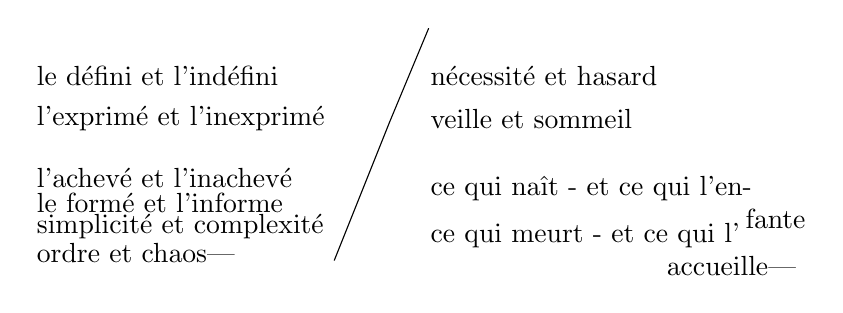
\begin{tikzpicture}[x=1cm,y=1cm]
\node[anchor=west] at (0,0) {le défini et l'indéfini};
\node[anchor=west] at (0,-.55) {l'exprimé et l'inexprimé};
\node[anchor=west] at (0,-1.3) {l'achevé et l'inachevé};
\node[anchor=west] at (0,-1.62) {le formé et l'informe};
\node[anchor=west] at (0,-1.92) {simplicité et complexité};
\node[anchor=west] at (0,-2.25) {\unsure{ordre et chaos}};
\draw (5.1,.6)--(4.6,-.6)--(3.9,-2.35);
\node[anchor=west] at (5,0) {nécessité et hasard};
\node[anchor=west] at (5,-.55) {veille et sommeil};
\node[anchor=north west,align=left] at (5,-1.15) {ce qui naît - et ce qui l'en-\\\hspace{4cm}fante};
\node[anchor=north west,align=left] at (5,-1.75) {ce qui meurt - et ce qui l'\\\hspace{3cm}\unsure{accueille}};
\end{tikzpicture}}

\scanpage{52}
% archive foliation: 51
\[
\underbrace{\Omega(\mathbb{R}^{n-1},\mathbb{R}^n)}_{1}\wedge\Omega(\mathbb{R}^n)\longrightarrow\Omega(\mathbb{R}^{n-1})\qquad\text{i.e.}
\]
\inserted{on choisit $\mathbb{R}^{n-1}\times\mathbb{R}^+$ comme $1/2$ espace de $\mathbb{R}^n$}
\[
\omega_n\xrightarrow{\sim}\omega_{n-1}
\]
compatible avec $\operatorname{Aut}(\mathbb{R}^{n-1},\mathbb{R}^n)={}$ssgrpe de $\mathrm{GL}(n,\mathbb{R})$ des matrices
\[
u_n:=\deleted{\unsure{\left(\begin{array}{c|c}u_{n-1}&\vdots\\\hline0&\lambda\end{array}\right)}}
\left(\begin{array}{c|c}
\begin{array}{c@{}c}\scriptstyle n-1\left\{\vphantom{\begin{matrix}a\\b\end{matrix}}\right.&\overbrace{u_{n-1}}^{n-1}\end{array}&\begin{matrix}\bullet\\\vdots\\\bullet\end{matrix}\\\hline
0\qquad0&\lambda
\end{array}\right)
\]
opérant sur $\omega_{n-1}$ par $\deleted{\unsure{\operatorname{sg}\det}}\varepsilon_{n-1}(u_{n-1})$, sur $\omega_n$ par $(\deleted{\unsure{\operatorname{sg}\det}}\inserted{\varepsilon_n}(u_n).\operatorname{sg}\lambda)\deleted{=\unsure{\operatorname{sg}\det u_{n-1}}}$
\[
\deleted{\unsure{\varepsilon_{n-1}(u_{n-1})}}
\]
\inserted{condition que l'application}
\[
\boxed{\varepsilon_n(u_n)=\operatorname{sg}(\lambda)\varepsilon_{n-1}(u_{n-1})}.
\]
\deleted{qui est donc \unsure{une condt satisfaite !}}

\deleted{Donc la donnée d'une théorie de \unsure{l'ori.} équivaut à la donnée de
\[
\left\{\begin{array}{ll}
(\varepsilon_n)_{n\in\mathbb{N}},&\text{où }\varepsilon_n:G_n\longrightarrow\{\pm1\}\\
(\unsure{s_n|\xi_n})_{n\in\mathbb{N}^*},&\text{où }\unsure{s_n|\xi_n}:\omega_n\xrightarrow{\sim}\omega_{n-1}
\end{array}\right\}
\]
(les iso $\omega_n\simeq\omega_{n-1}$, et $\omega_0\simeq\{\pm1\}$, donnent $\omega_n\simeq\{\pm1\}$)}

Ceci détermine $\varepsilon_1:\mathbb{R}^*\longrightarrow\{\pm1\}$ par
\[
\varepsilon_1=\operatorname{sg}:\mathbb{R}^*\longrightarrow\{\pm1\}
\]
et pr \unsure{dim|des} plus gén., par récurrence
\[
\varepsilon_n(u)=\operatorname{sg}\circ\det(u)\qquad u\in\mathrm{GL}(n,\mathbb{R})
\]

\deleted{\illegible{1}}
\figure{\begin{tikzpicture}\draw (0,0)--(.75,0);\draw (.08,-.12)--(.75,-.12);\end{tikzpicture}}

\scanpage{53}
% archive foliation: 52
\mspage{82}
XVIII\qquad L e s\quad é p o u s a i l l e s\qquad (2)

J'ai scruté et j'ai fouillé - par pleines brassées je ramasse tout à l'entour les paires enlacées disant un même message. Pêle-mêle je les jette devant moi ...

Puis, comme un enfant appliqué intensément enfile collier de pierres multicolores qu'il assemble à son gré - sans en laisser une seule, car toutes lui semblent belles ! ... lestement passant les unes, et sur d'autres s'arrêtant longement pour les contempler à loisir ... ainsi du chaos chatoyant de mes trouvailles je prépare ce collier - m o n collier - pour te l'offrir ... et \deleted{pour} l'oublier ...

Le jeu était p l a i s i r - il était découverte ! Qu'importe s'il reste \deleted{collier}\inserted{trace} pour témoigner du jeu \inserted{révolu} d'un enfant qui découvre \unsure{!} Quel sens a un collier, si ce n'est le plaisir de le faire ...

Ou ... susciter en \uline{toi} \unsure{désir}\deleted{\unsure{i r}} de scruter et fouiller - de ramasser toi-même perles et pierres par poignées ... contempler longuement une à une celles qui t e parlent, et au gré de \deleted{ta} \inserted{\uline{ton} « \deleted{\unsure{désir}}\inserted{désir} \unsure{»}} \deleted{fantaisie} assembler t o n collier ?

\margin{\figure{\begin{tikzpicture}\draw (.05,1.2) .. controls (.13,.8) and (-.07,.35) .. (0,.1) --(.38,0);\end{tikzpicture}}}

\deleted{A quoi bon un collier qui ne suscite désir d'en faire un plus beau ?}

\margin{\figure{\begin{tikzpicture}\draw (.38,1)--(0,1)--(0,0);\end{tikzpicture}}}
Je termine d'un deuxième rang de paires enlacées \unsure{...} \unsure{Si} le jeu \unsure{te} plait encore, \deleted{tu peux} regarde\deleted{r} faire - ou \deleted{tu peux} fai\deleted{re}\inserted{s-en \deleted{\illegible{2}}\inserted{un plus beau !}}

11. En les choses de la Création s'enlacent et s'unissent :

\begin{flushleft}
l u m i è r e\quad et\quad o m b r e\\
le clair et l'obscur\\
le jour et la nuit\\
le brillant et le terne

savoir et mystère\\
le connu et l'inconnu\\
le connaissable et l'inconnaissable\\
connaissance et ignorance

le précis et le vague\\
le particulier et le général
\end{flushleft}

\figure{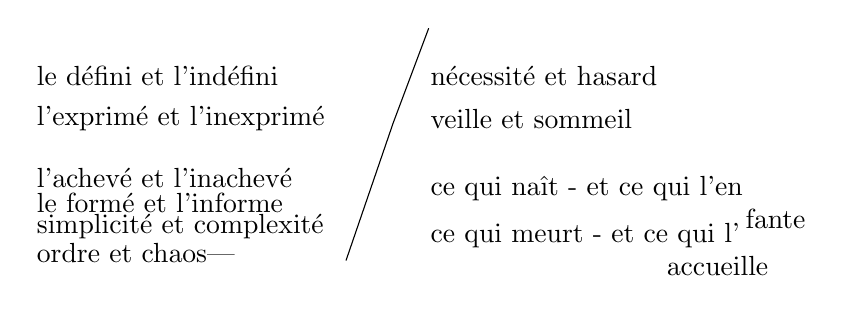
\begin{tikzpicture}[x=1cm,y=1cm]
\node[anchor=west] at (0,0) {le défini et l'indéfini};
\node[anchor=west] at (0,-.55) {l'exprimé et l'inexprimé};
\node[anchor=west] at (0,-1.3) {l'achevé et l'inachevé};
\node[anchor=west] at (0,-1.62) {le formé et l'informe};
\node[anchor=west] at (0,-1.92) {simplicité et complexité};
\node[anchor=west] at (0,-2.25) {\unsure{ordre et chaos}};
\draw (5.1,.6)--(4.65,-.6)--(4.05,-2.35);
\node[anchor=west] at (5,0) {nécessité et hasard};
\node[anchor=west] at (5,-.55) {veille et sommeil};
\node[anchor=north west,align=left] at (5,-1.15) {ce qui naît - et ce qui l'en\\\hspace{4cm}fante};
\node[anchor=north west,align=left] at (5,-1.75) {ce qui meurt - et ce qui l'\\\hspace{3cm}accueille};
\end{tikzpicture}}

\scanpage{54}
% archive foliation: 53
\[
U\underset{\omega'}{\underbrace{\subset}}W\underset{\omega}{\underbrace{\subset}}V
\qquad\Omega(V/W)\wedge\Omega(V)\longrightarrow\Omega(W)
\]
\[
\mathrm{St}_{\omega}:\Omega(V)\unsure{\longrightarrow|\text{---}}\Omega(W)
\]
\[
\mathrm{St}_{\omega'}:\Omega(W)\text{---}\Omega(U)
\]
\[
\mathrm{St}_{\omega'}\mathrm{St}_{\omega}:\Omega(V)\longrightarrow\Omega(U)
\]
\[
I(\omega,\omega')\in\Omega
\]
\margin{$(\omega,\omega')\longmapsto\omega\times\omega'$}
\[
\Omega(V)\wedge\Omega(V')\longrightarrow\Omega(V\unsure{\wedge|\times}V')
\]
\[
\omega'\times\omega=(-1)^{\dim V.\dim V'}\deleted{\unsure{\Omega}}\omega\times\omega'
\]
\[
\deleted{\mathrm{St}(\omega)=\mathrm{St}(\omega')}
\]
\diagram{\begin{tikzcd}[column sep=small,row sep=small]
\mathbb{R}\arrow[d,phantom,"\cup"]\arrow[r,phantom,"\subset"] &
\mathbb{R}^2\arrow[d,phantom,"\cup"]\arrow[r,phantom,"\subset"] &
\mathbb{R}^3\arrow[d,phantom,"\cup"]\arrow[r,dash] &
\mathbb{R}^{n-1}\arrow[d,phantom,"\cup"]\arrow[r,phantom,"\subset"] &
\mathbb{R}^n\arrow[d,phantom,"\cup"]\\
\mathbb{R}^+\arrow[r,phantom,"\subset"] &
\mathbb{R}\times\mathbb{R}^+\arrow[r,phantom,"\subset"] &
\mathbb{R}^2\times\mathbb{R}^+\arrow[r,phantom,"\subset"] &
\mathbb{R}^{\unsure{n-2}}\times\mathbb{R}^+\arrow[r,phantom,"\subset"] &
\mathbb{R}^{n-1}\times\mathbb{R}^+
\end{tikzcd}}
\[
\unsure{\ell_1\wedge\text{---}\ell_{n-1}\wedge\ell_n|e_1\wedge\text{---}e_{n-1}\wedge e_n}
\qquad e_1\wedge\text{---}\wedge e_{n-1}\wedge e_n
\]
\[
\omega\times\omega'\qquad I(\omega,\omega')\qquad I(\omega',\omega)
\]
\[
\left\{\begin{array}{l}
\mathrm{St}(\omega\times\omega')=\inserted{\unsure{(-1)^q|(-1)^{?}}}\mathrm{St}(\omega)\times\omega'\\
\mathrm{St}(\omega\times\omega')=\deleted{\unsure{(-1)^p}}\omega\times\mathrm{St}\omega'
\end{array}\right.
\]
\[
\underbrace{e_1\text{---}e_p}\quad f_1\text{---}f_q
\]
\[
\mathrm{St}(e_1\text{---}e_{p-1}e_p f_1\text{---}f_q)
=(-1)^{\unsure{q}}e_1\text{---}e_{p-1}\widehat e_p f_1\unsure{\text{---}f_q}
\]
\[
e_1\ e_2\text{---}e_n
\]
\figure{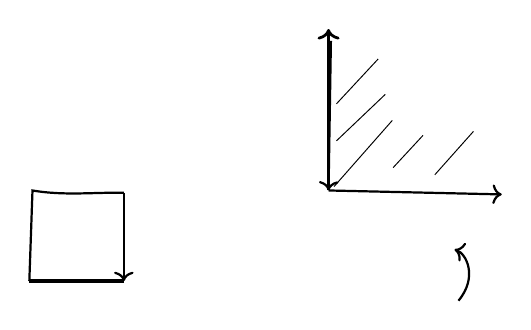
\begin{tikzpicture}[x=1cm,y=1cm]
\draw[line width=.8pt] (0,0)--(.04,1.15) .. controls (.45,1.08) and (.83,1.13) .. (1.2,1.12);
\draw[line width=.8pt,->] (1.2,1.12)--(1.2,0);
\draw[line width=1.2pt] (1.2,0)--(0,0);
\draw[line width=1pt,->] (3.8,1.15)--(3.8,3.2);
\draw[line width=.8pt,->] (3.83,3.05)--(3.8,1.15);
\draw[line width=.8pt,->] (3.8,1.15)--(6,1.1);
\draw[line width=.35pt] (3.9,2.25)--(4.43,2.82);
\draw[line width=.35pt] (3.9,1.78)--(4.52,2.37);
\draw[line width=.35pt] (3.87,1.2)--(4.61,2.04);
\draw[line width=.35pt] (4.62,1.44)--(5,1.85);
\draw[line width=.35pt] (5.15,1.35)--(5.64,1.9);
\draw[line width=.8pt,->] (5.45,-.25) .. controls (5.7,.05) and (5.55,.35) .. (5.4,.4);
\end{tikzpicture}}

\scanpage{55}
% archive foliation: 54
\margin{\illegible{1}}
XVIII\qquad L e s\quad é p o u s a i l l e s\qquad (2)

J'ai scruté et j'ai fouillé - par pleines brassées je ramasse tout à l'entour les paires enlacées disant un même message. Pêle-mêle je les jette devant moi ...

Puis, comme un enfant appliqué intensément enfile collier de pierres multicolores qu'il \unsure{assem\deleted{t}ble} à son gré - sans en laisser une seule, car toutes lui semblent belles ! ... lestement passant les unes, et sur d'autres s'arrêtant longement pour les contempler à loisir ... ainsi du chaos chatoyant de mes trouvailles je prépare ce collier - m o n collier - pour te l'offrir ... et \deleted{pour} l'oublier ...

Le jeu était p l a i s i r - il était découverte ! Qu'importe s'il reste \deleted{\unsure{collier}} \inserted{trace} pour témoigner du jeu \inserted{révolu} d'un enfant qui découvre \unsure{!} Quel sens a un collier, si ce n'est le plaisir de le faire ...

Ou ... susciter en \uline{toi} d é s i r de scruter et fouiller - de ramasser toi-même perles et pierres par poignées ... contempler longuement une à une celles qui t e \unsure{s} parlent, et au gré de \deleted{ta} \inserted{\uline{ton} « \unsure{désir} »} \deleted{fantaisie} assembler t o n collier ?

\deleted{A quoi bon un collier qui ne suscite désir d'en faire un plus beau ?}

Je termine d'un deuxième rang de paires enlacées ... \unsure{Si} le jeu \unsure{te} plait encore, \deleted{tu peux} regarde\deleted{r} faire ... ou \deleted{tu peux} fai\deleted{re}\inserted{s} \inserted{en un plus beau.}

11. En les choses de la Création s'enlacent et s'unissent :

\begin{flushleft}
l u m i è r e\quad et\quad o m b r e\\
le clair et l'obscur\\
le jour et la nuit\\
le brillant et le terne

savoir et mystère\\
le connu et l'inconnu\\
le connaissable et l'inconnaissable\\
connaissance et ignorance

le précis et le vague\\
le particulier et le général
\end{flushleft}

\figure{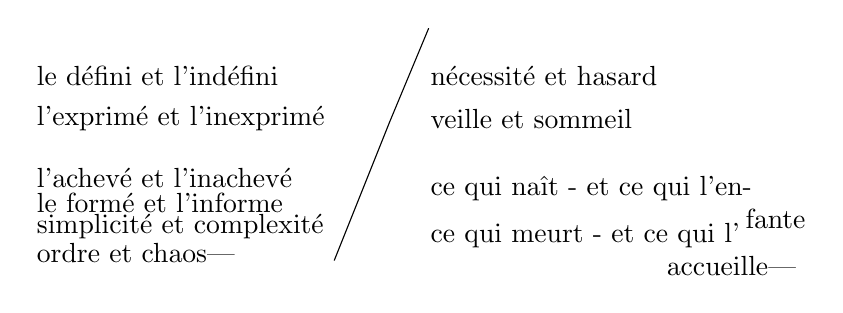
\begin{tikzpicture}[x=1cm,y=1cm]
\node[anchor=west] at (0,0) {le défini et l'indéfini};
\node[anchor=west] at (0,-.55) {l'exprimé et l'inexprimé};
\node[anchor=west] at (0,-1.3) {l'achevé et l'inachevé};
\node[anchor=west] at (0,-1.62) {le formé et l'informe};
\node[anchor=west] at (0,-1.92) {simplicité et complexité};
\node[anchor=west] at (0,-2.25) {\unsure{ordre et chaos}};
\draw (5.1,.6)--(4.6,-.6)--(3.9,-2.35);
\node[anchor=west] at (5,0) {nécessité et hasard};
\node[anchor=west] at (5,-.55) {veille et sommeil};
\node[anchor=north west,align=left] at (5,-1.15) {ce qui naît - et ce qui l'en-\\\hspace{4cm}fante};
\node[anchor=north west,align=left] at (5,-1.75) {ce qui meurt - et ce qui l'\\\hspace{3cm}\unsure{accueille}};
\end{tikzpicture}}

\scanpage{56}
% archive foliation: 55
$k$ anneau comm.

$\mathcal V=\mathcal V(k)$ catégorie des Modules libres de type fini sur $k$ (morphismes : \uline{iso})
\[
\begin{array}{c}
\text{''}\\
\displaystyle\coprod_{n\in\mathbb{N}}\mathcal V_n(k)
\end{array}
\qquad\mathcal V_n(k)\quad\text{catégorie des modules libres de rang }n\text{ sur }k
\]

$\mathcal V$ catégorie additive (graduée)

\deleted{a) $\mathcal V\xrightarrow{\Delta}\unsure{\mathcal V_1}$ foncteur}

\deleted{b) $\unsure{\Delta|\Delta_2}$} $P(k)$ catégorie de Picard des $k$-modules libres de rang $1$ $\mathbb{Z}$-gradués, avec donnée de comm. l'isomorphisme de Koszul

\uline{Théorie des \inserted{modules} déterminants gradués}

a) $\mathcal V\xrightarrow{\Delta}P$ $\otimes$ foncteur [donc muni d'iso funct.
\[
\Delta(V+V')\overset{\varphi_{V,V'}}{\simeq}\Delta(V)\otimes\Delta(V')
\]
\[
(\Rightarrow\Delta(0)\simeq\mathbf1\quad\text{can}^{\mathrm t})
\]
\deleted{\unsure{gr}}

b)\deleted{\unsure{a)}} Si $\operatorname{rg}(V)=1$, $\Delta(V)\simeq V$, de degré $1$.

c) Soient $V\supset W_1$ ; $W_2,W_2'$ deux suppl. de $W_1$ dans $V$ ($W_1,W_2$ libres, donc $V,W_2'$ aussi)
\[
\begin{array}{l}
\alpha:W_1+W_2\xrightarrow{\sim}V\\
\alpha':W_1+W_2'\xrightarrow{\sim}V\\
\lambda:W_2\simeq W_2'
\end{array}
\]
\diagram{\begin{tikzcd}[column sep=small,row sep=large]
\Delta(W_1+W_2)\arrow[r,"{\substack{\Delta(\alpha)\\\sim}}"]\arrow[d,dash,"{\varphi_{W_1,W_2}}"',"\sim"{rotate=90}] &
\Delta(\unsure{W|V}) &
\Delta(W_1+W_2')\arrow[l,"{\substack{\Delta(\alpha')\\\sim}}"']\arrow[d,dash,"{\varphi_{\unsure{W_2|W_1},W_2'}}","\sim"'{rotate=90}]\\
\Delta(V_1)\otimes\Delta(W_2) &&
\Delta(W_1)\otimes\Delta(W_2')\arrow[ll,"{\substack{\operatorname{id}\otimes\Delta(\lambda)\\\sim}}"]
\end{tikzcd}}

commutatif.

[ Equivaut à : Si $u$ est un autom de $V$ qui est l'identité sur $W_1$ et sur $V/W_1\ (\simeq W_2)$, alors $\Delta(u)=\operatorname{id}_{\Delta(V)}$ ]

\end{document}
